%!TEX root = presentation.tex
\section{Current state}

\begin{frame}
	\frametitle{Current state}
	\begin{columns}
		\begin{column}{0.6\textwidth}
			\begin{itemize}
				\item Language layer implemented and working
				\item Runtime layer: Execution on Stratosphere with iteration and convergence support
				\item Implemented algorithms: PageRank, NNMF and K-means
			\end{itemize}
		\end{column}
		\begin{column}{0.4\textwidth}
			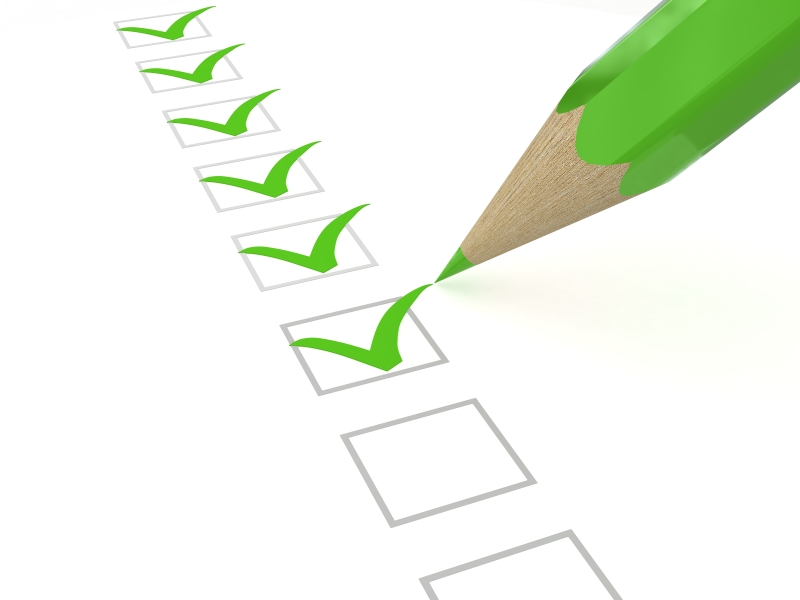
\includegraphics[width=\textwidth]{images/checklist.jpg}
		\end{column}
	\end{columns}
\end{frame}

\begin{frame}
	\frametitle{Live demonstration}
	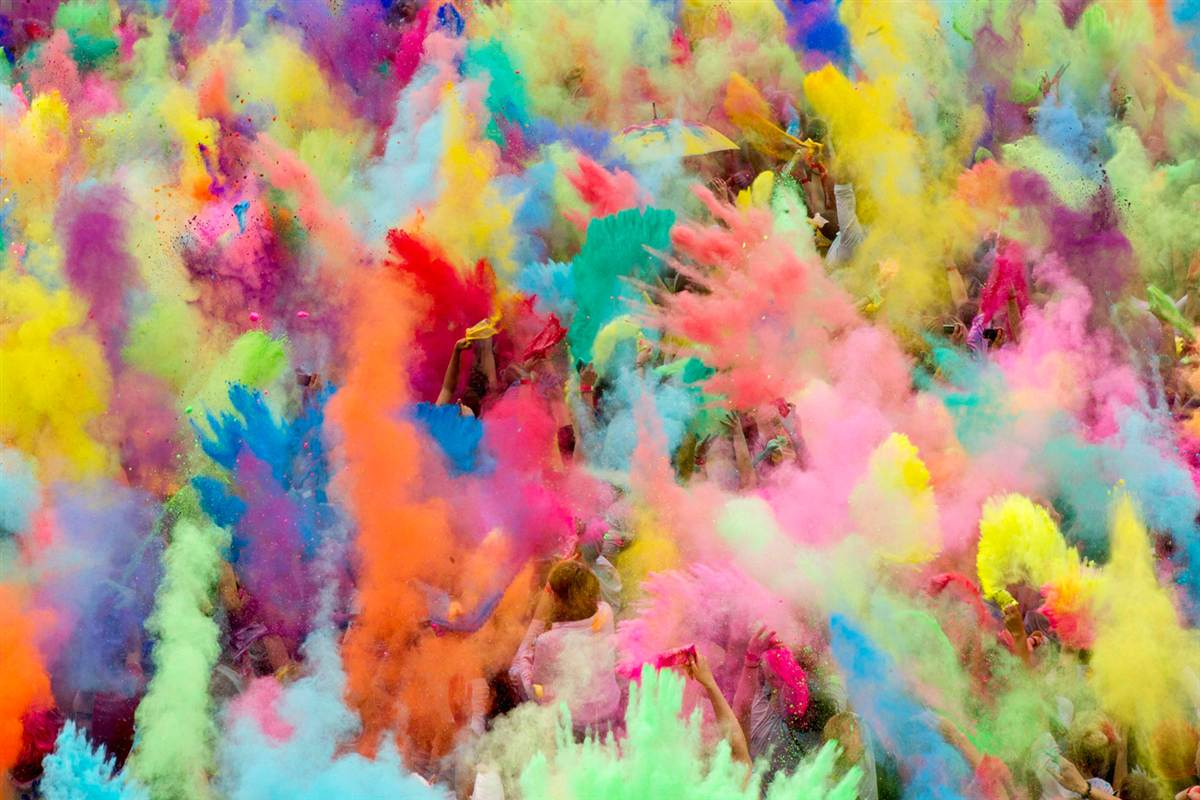
\includegraphics[width=\textwidth]{images/holi.jpg}
\end{frame}